\section{Mission frontend}

Pendant mon alternance liée au projet Pipeline documentaire, j'ai également travaillé sur une mission frontend. Ma responsabilité était de transformer la page d'importation des fichiers de transactions de carburant dans le projet Gestion de parc. Cette transformation a impliqué les modifications suivantes :

\begin{itemize}
    \item Réorganisation de l'emplacement du bouton de téléchargement de fichiers et du bouton d'importation.
    \item Ajout d'un bouton pour afficher une fenêtre modale.
    \item Intégration de la fenêtre modale affichant un guide sur la manière de télécharger les fichiers de transaction de carburant à partir des sites web des différents prestataires.
    \item Adaptation de la page afin qu'elle communique avec le Pipeline documentaire au lieu de l'ancienne API pour certains types de fichiers de transactions de carburant.
    \item Affichage de messages sur l'état de l'importation tout au long du processus.
\end{itemize}

La raison derrière cette mission était que selon les retours des utilisateurs, la page d'origine dédiée à l'importation des fichiers de transactions de carburant manquait de convivialité et ne répondait pas aux attentes de leur expérience. Ils ne savaient souvent pas où obtenir les fichiers de transactions de carburant, et lorsqu'ils importaient un fichier via la page, ils ne savaient pas si l'importation avait réussi ou échoué, et en cas d'échec, ils ne comprenaient pas pourquoi. Cela peut être vu sur la version originale de la page d'importation (Figure~\ref{fig:original-import-page}).

\begin{figure}[ht]
    \centering
    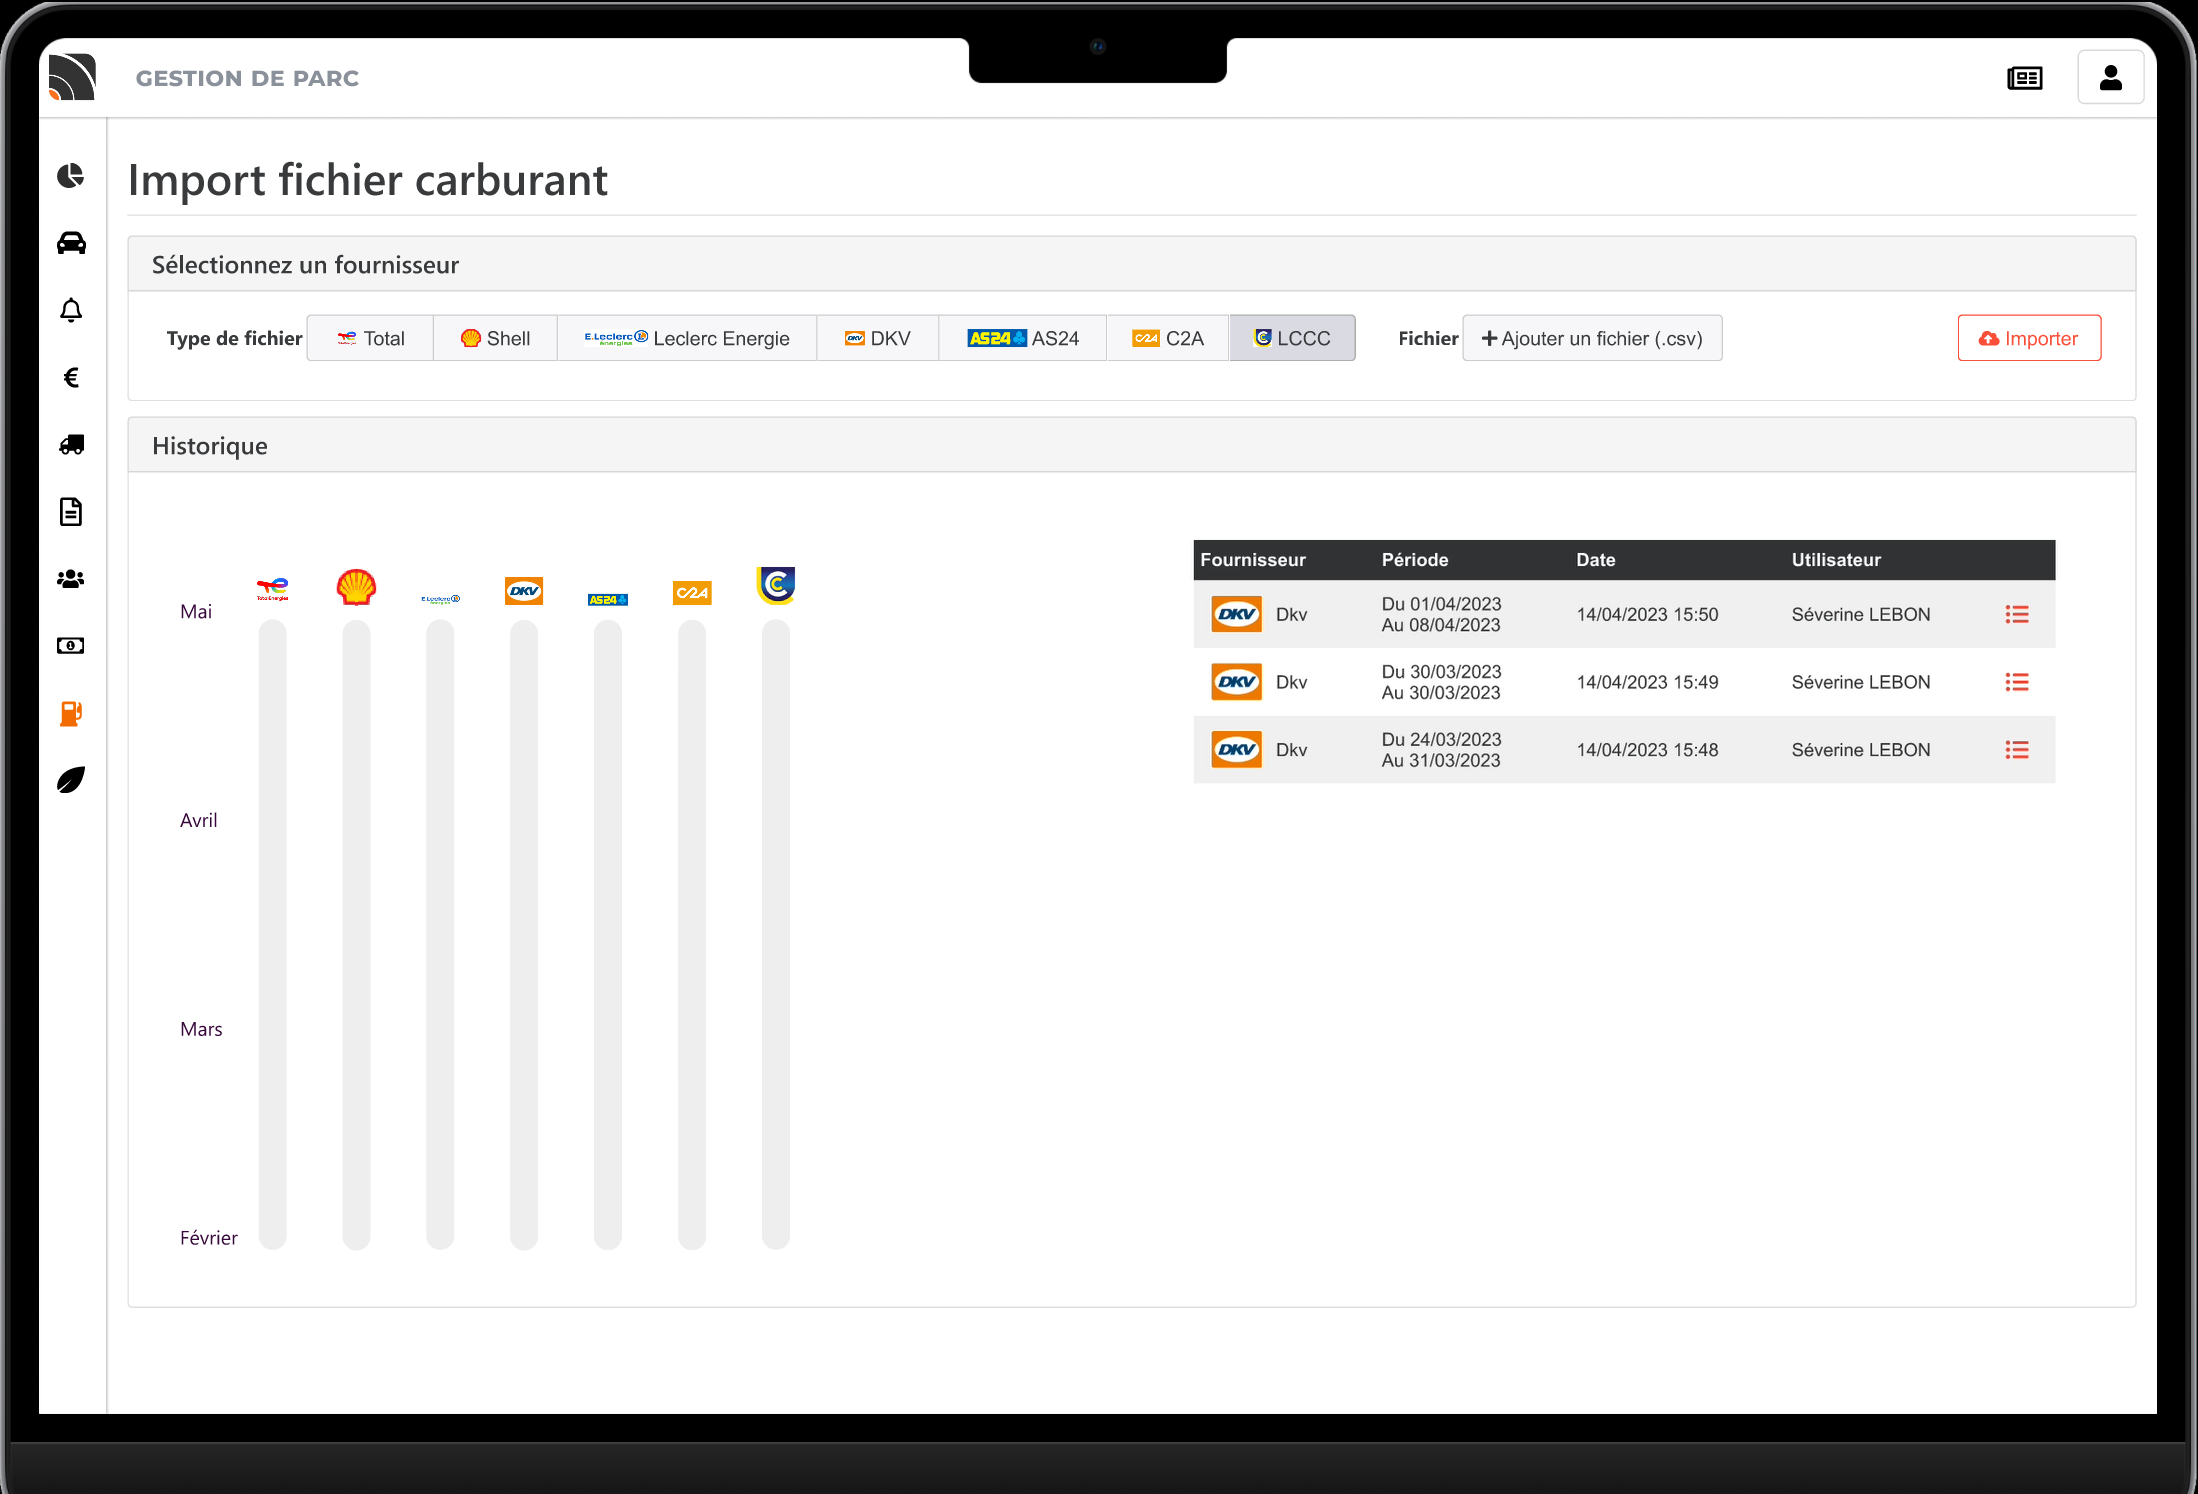
\includegraphics[width=0.73\textwidth]{img/frontend-maquettage-original}
    \caption{La version originale de la page d'importation des fichiers de transaction de carburant.}
    \label{fig:original-import-page}
\end{figure}

Pour accomplir cette mission, j'ai tout d'abord dû créer une maquette de la nouvelle apparence de la page, en tenant compte des exigences. Après quelques ajustements issus de discussions avec le propriétaire du produit, la version finale de la maquette a été approuvée, me permettant ainsi de débuter sa mise en œuvre. Dans cette section, je vais présenter les détails de la maquette que j'ai élaboré, ainsi que la mise en œuvre technique des modifications.

\subsection{Maquettage}

Les figures suivantes illustrent différents aspects de la maquette : la réorganisation des boutons et l'ajout du bouton \foreignquote{french}{Guide de téléchargement} (Figure~\ref{fig:frontend-maquettage-total-buttons}), l'intégration de la fenêtre modale (Figure~\ref{fig:frontend-maquettage-total-modal}), ainsi que la présentation des retours à l'utilisateur en cas de succès ou d'erreur et leur séquence (Figure~\ref{fig:frontend-maquettage-total-file-sent}, Figure~\ref{fig:frontend-maquettage-feedbacks}). J'ai créé cette maquette interactive dans Figma et elle est disponibles sur le lien \url{https://figma.fun/kIw9mt}.

\begin{figure}[ht]
    \centering
    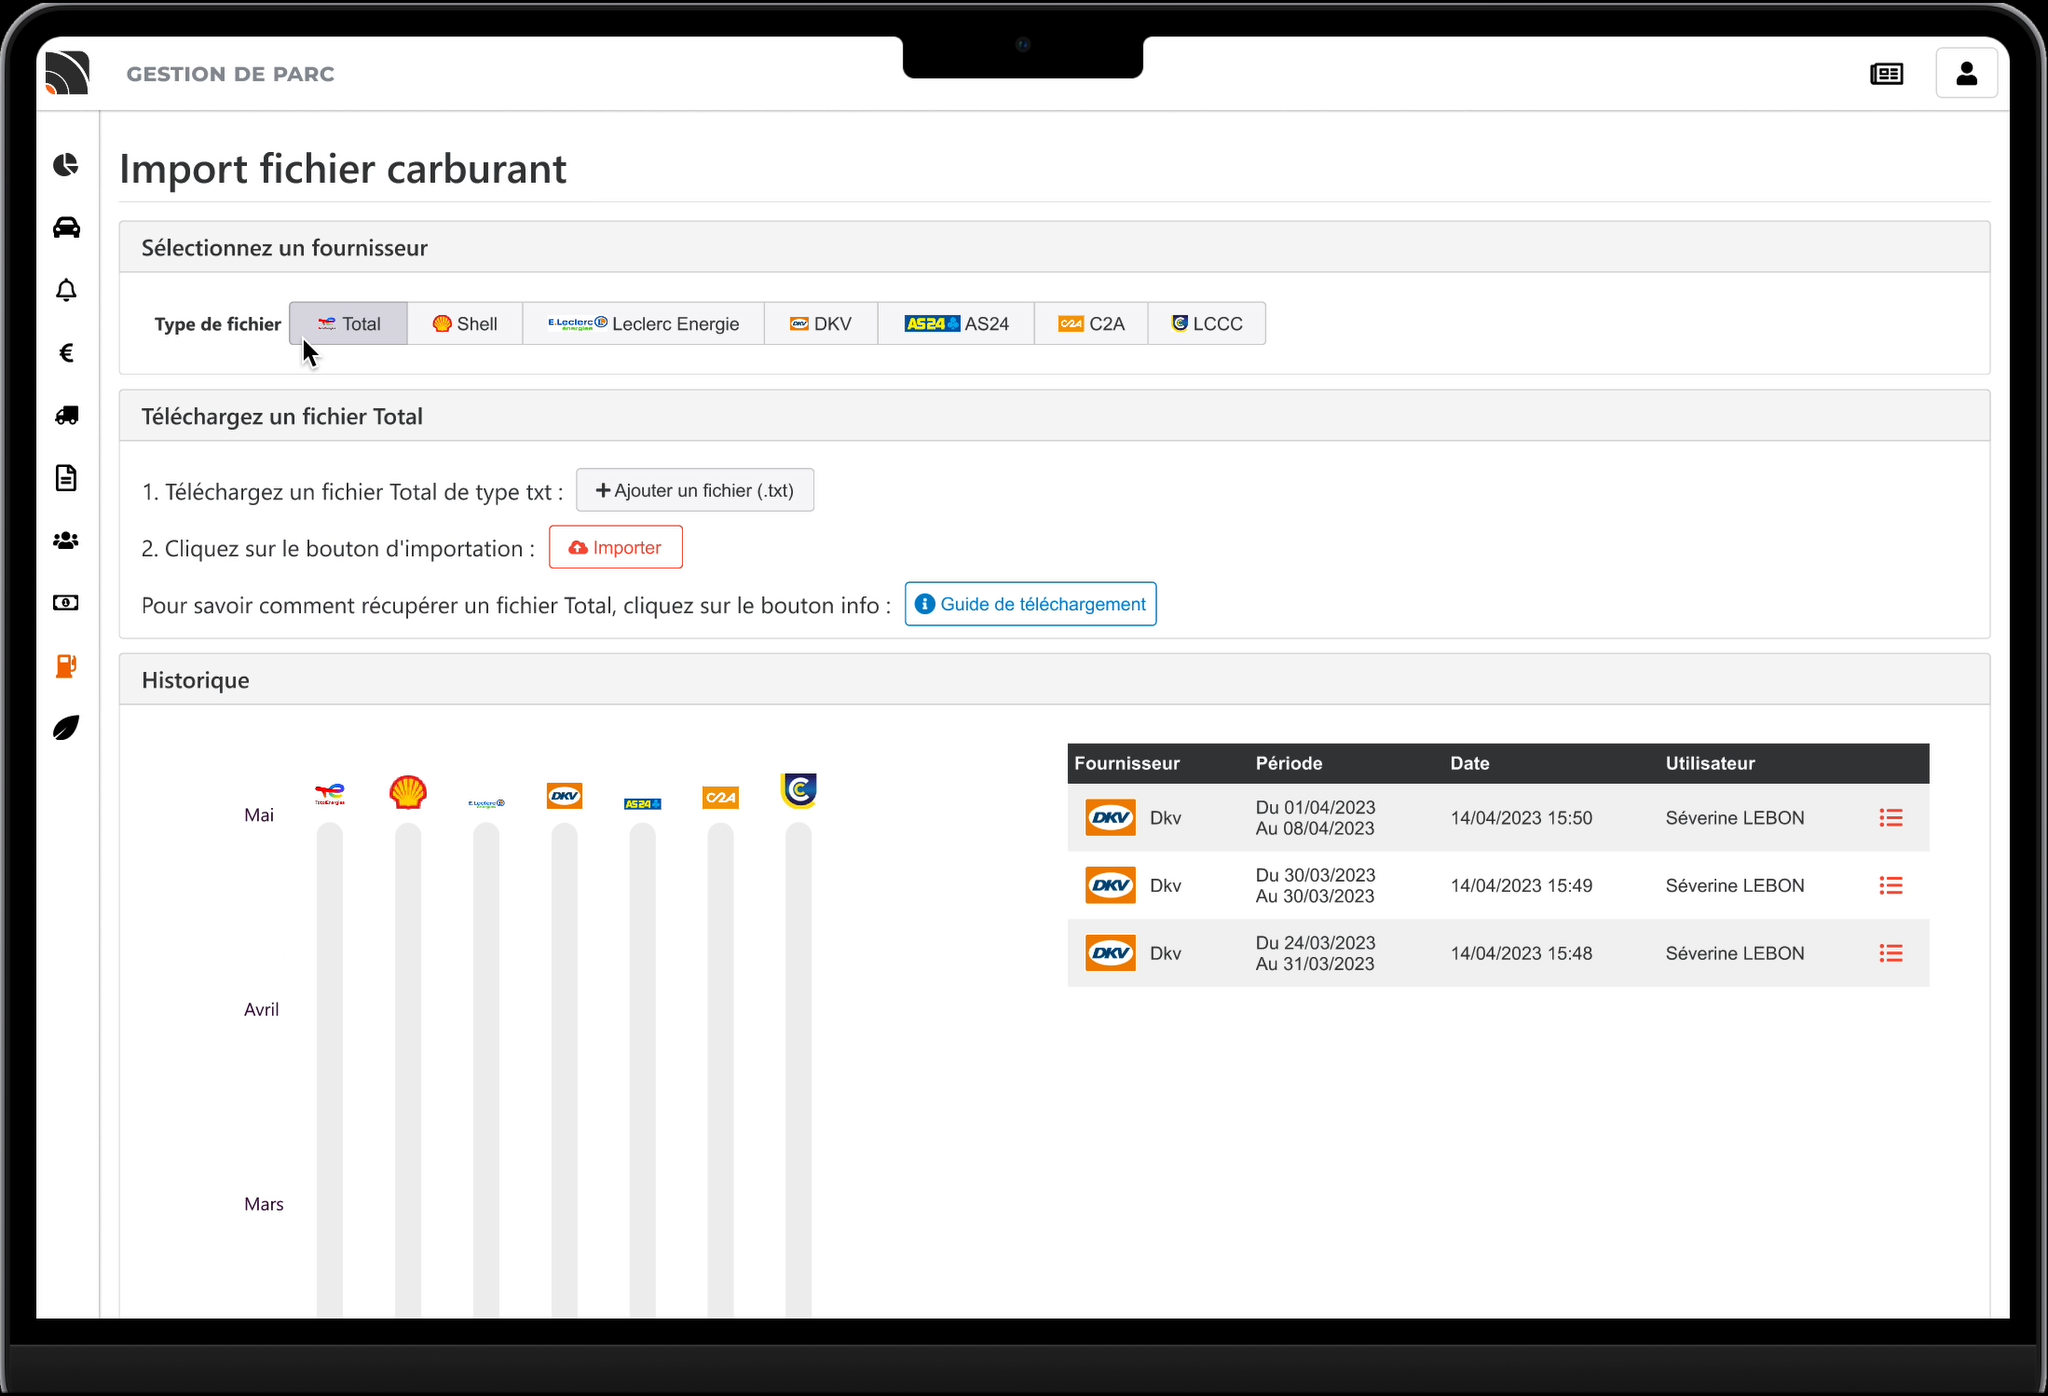
\includegraphics[width=0.73\textwidth]{img/frontend-maquettage-total-buttons}
    \caption{La maquette de la page d'importation des fichiers de transaction de carburant avec le placement réorganisé des boutons et le bouton Guide de téléchargement ajouté.}
    \label{fig:frontend-maquettage-total-buttons}
\end{figure}

\begin{figure}[ht]
    \centering
    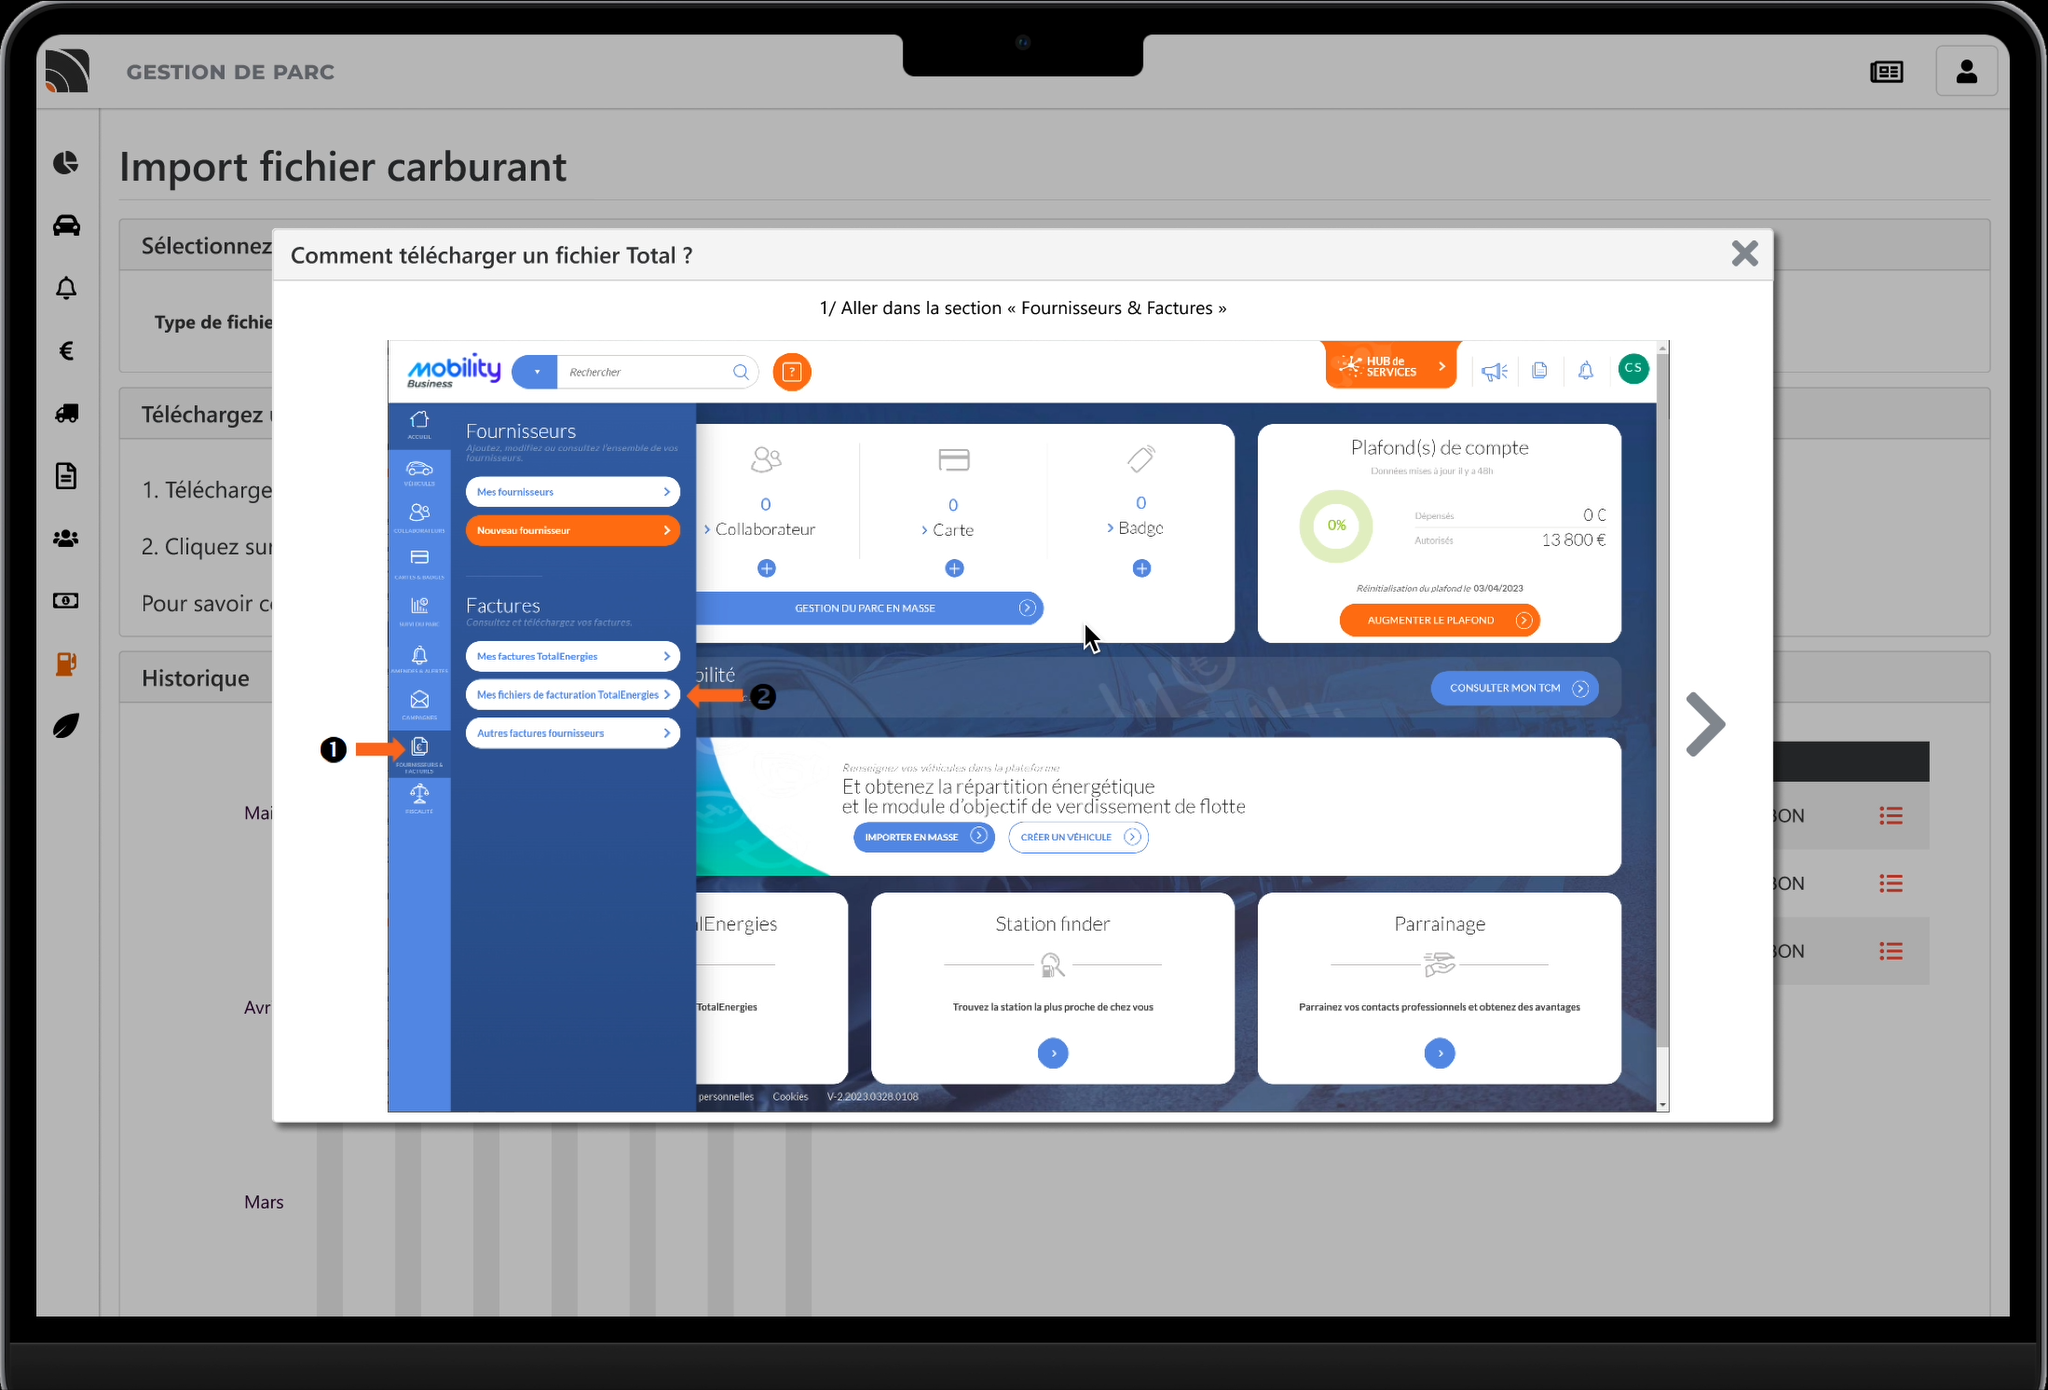
\includegraphics[width=\textwidth]{img/frontend-maquettage-total-modal}
    \caption{La maquette de la page d'importation des fichiers de transaction de carburant avec la fenêtre modale.}
    \label{fig:frontend-maquettage-total-modal}
\end{figure}

\begin{figure}[ht]
    \centering
    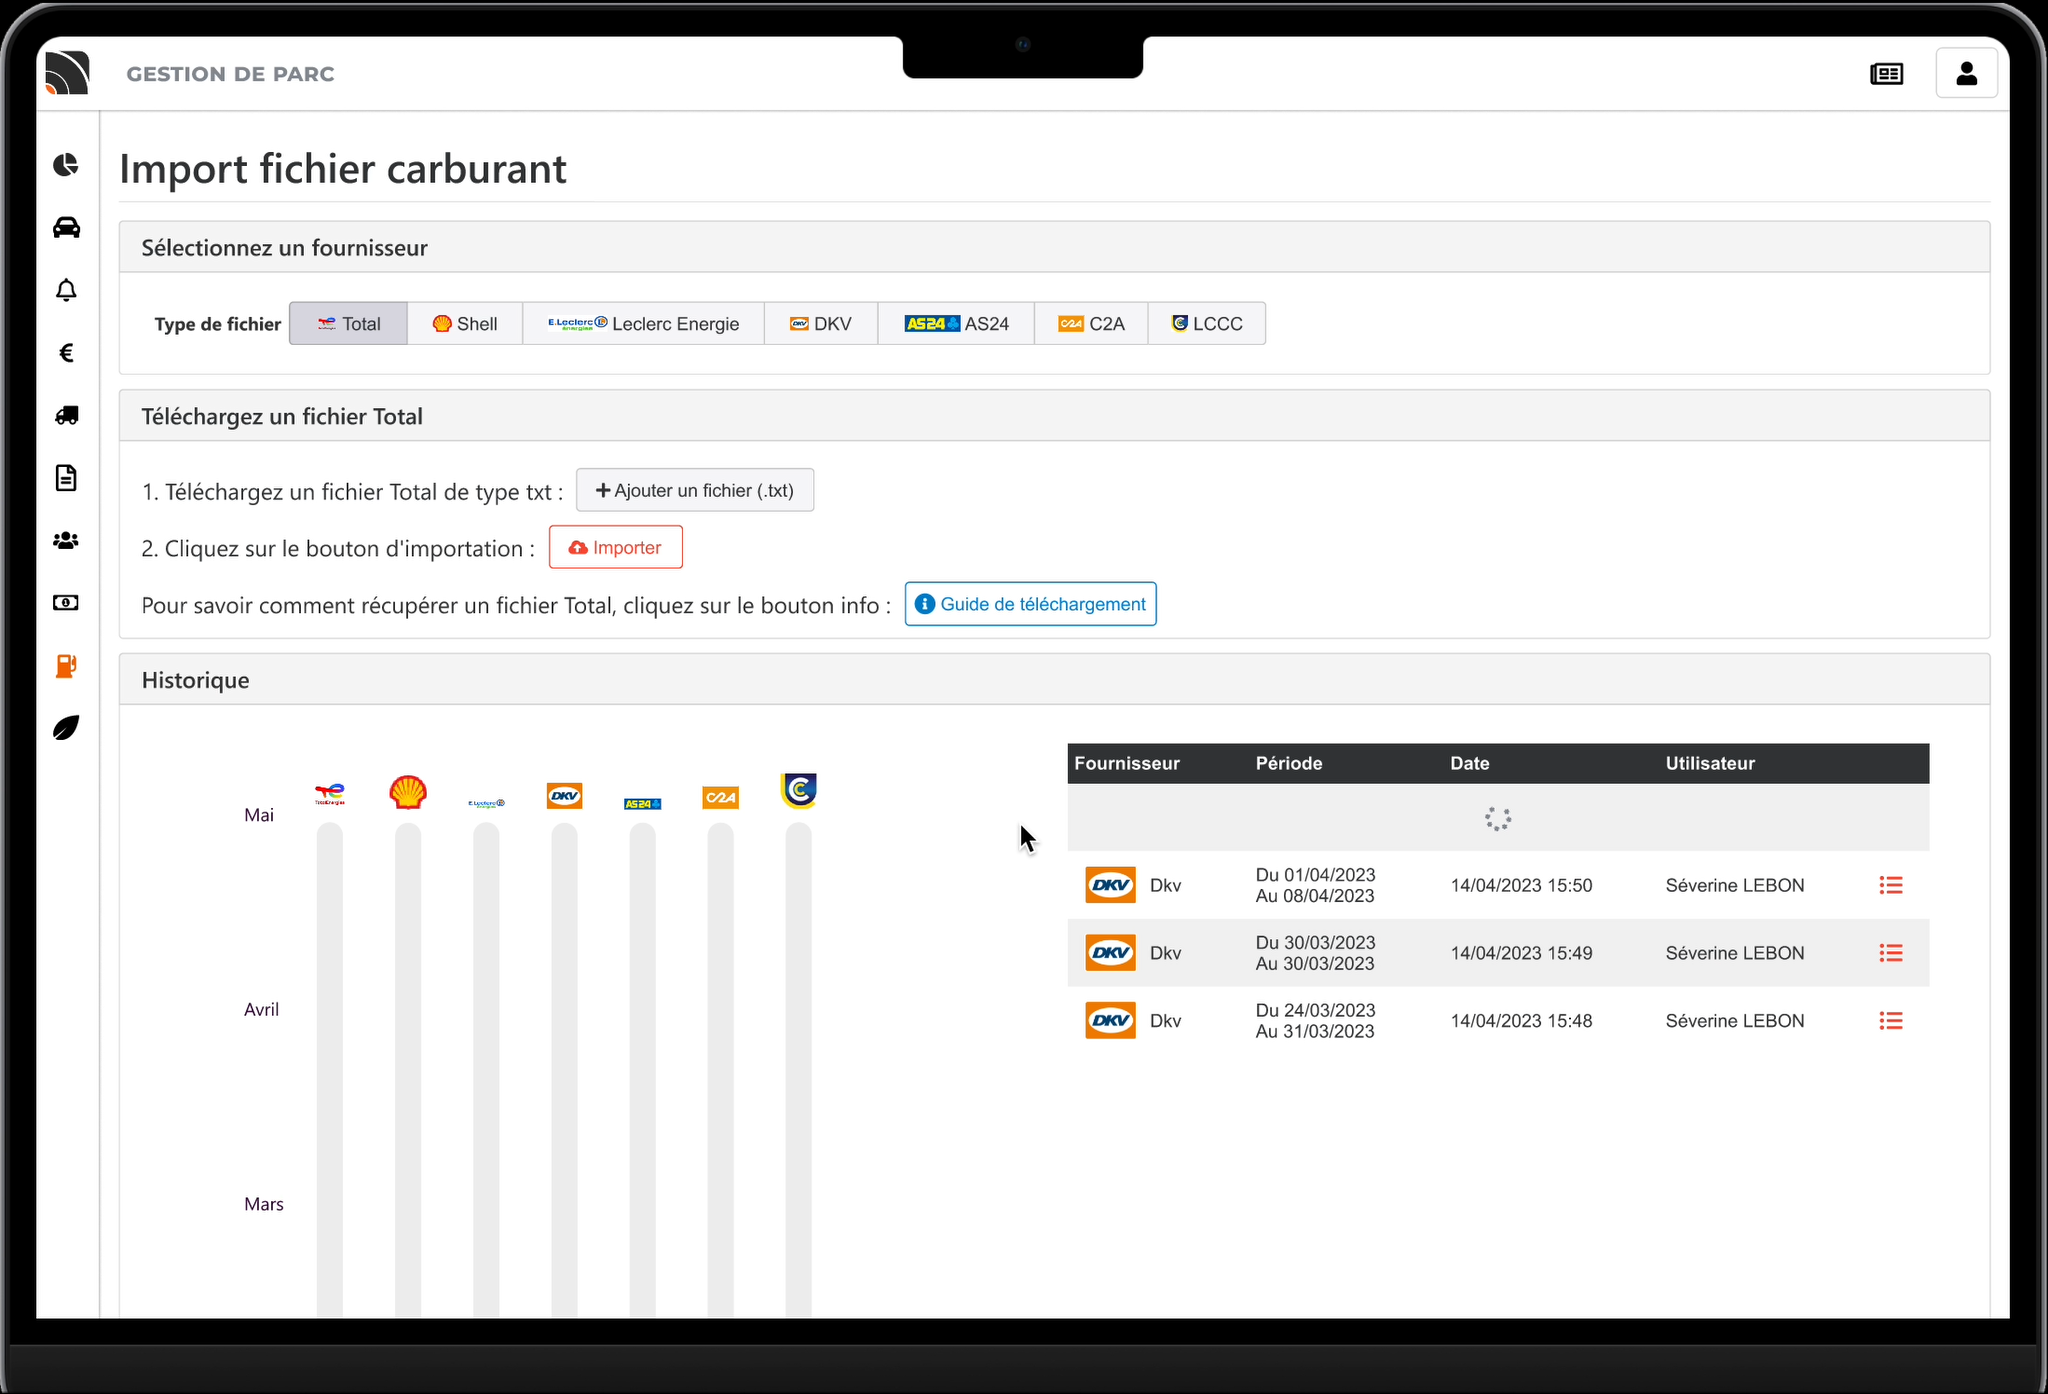
\includegraphics[width=\textwidth]{img/frontend-maquettage-total-file-sent}
    \caption{La maquette de la page d'importation des fichiers de transaction de carburant. Après avoir cliqué sur le bouton d'importation, l'utilisateur reçoit un retour indiquant que le fichier a été envoyé pour être importé.}
    \label{fig:frontend-maquettage-total-file-sent}
\end{figure}

\begin{figure}[ht]
    \centering
    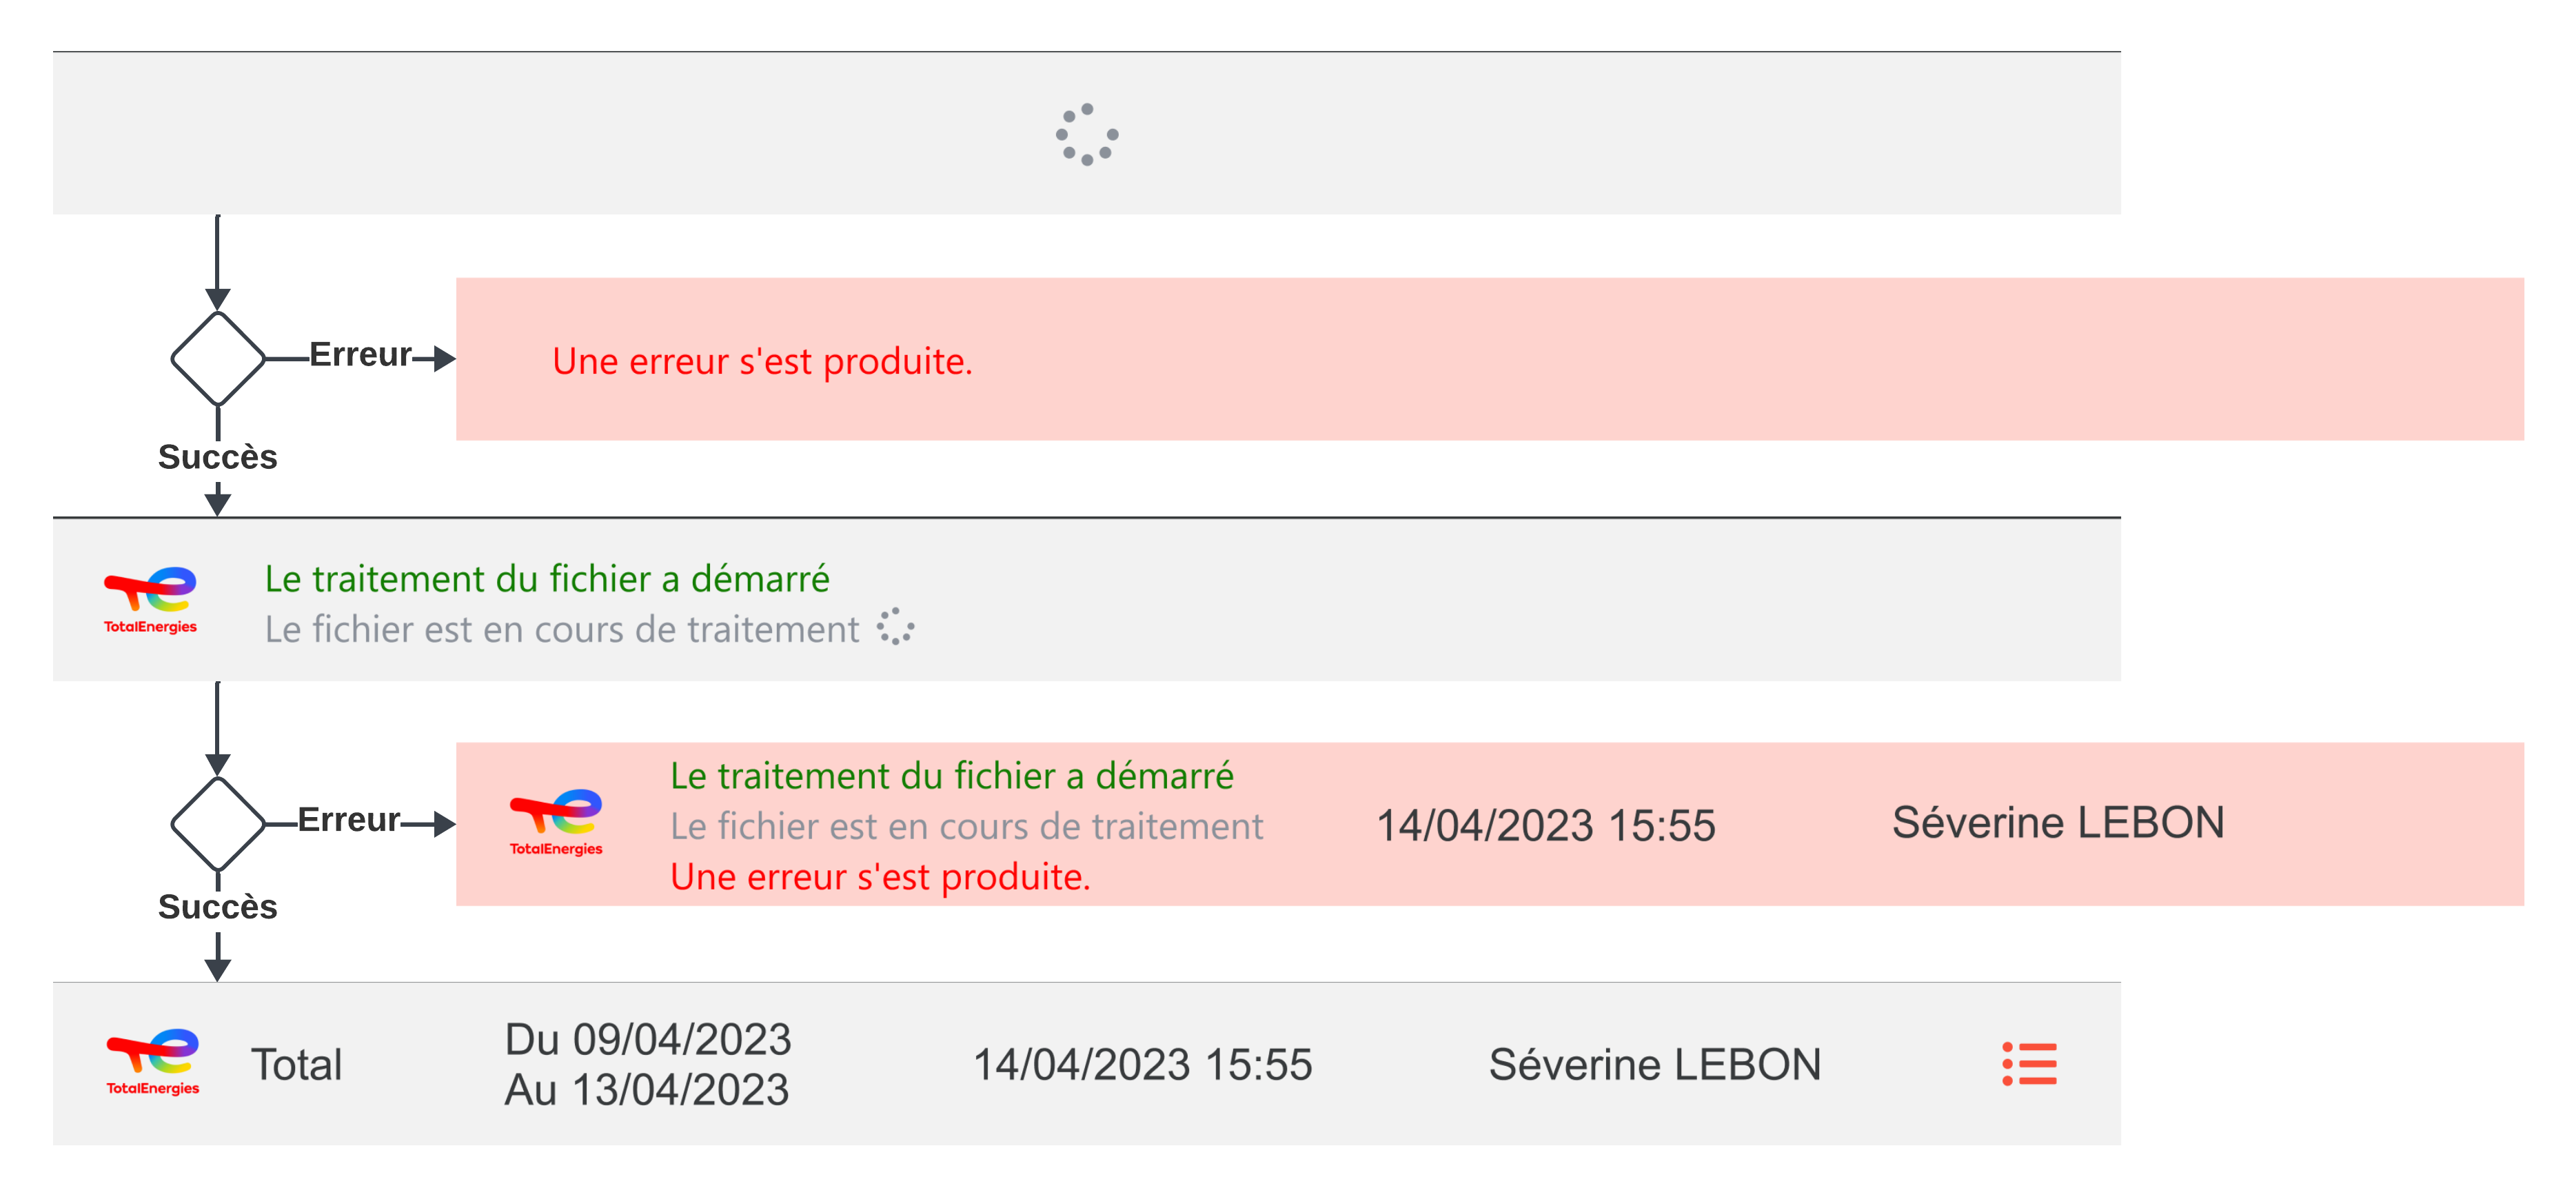
\includegraphics[width=\textwidth]{img/feedbacks}
    \caption{Série de retours à l'utilisateur sur l'état de l'importation du fichier.}
    \label{fig:frontend-maquettage-feedbacks}
\end{figure}

\subsection{Développement frontend}

Pour mettre en œuvre les modifications qui ont été visuellement conçues dans la maquette, j'ai dû modifier le fichier \Verb|import.blade.php| dans le dossier \Verb|Suivideflotte/Fleet/Packages/Fuel/resources/views| du projet Portail, qui comprend le projet Gestion de parc (Fleet) (Figure~\ref{fig:architecture}, page~\pageref{fig:architecture}). Les principales modifications que j'ai apportées sont les suivantes :

\begin{itemize}
    \item J'ai modifié le formulaire d'importation de fichiers d'origine. J'ai vidé la route d'action du formulaire, car elle sert désormais uniquement à sélectionner un prestataire et non à télécharger un fichier, l'action du formulaire étant gérée par JavaScript (Code source~\ref{code:frontend-diff-original-form}).
    \item J'ai ajouté un nouveau formulaire de téléchargement de fichier pour permettre aux utilisateurs de télécharger des fichiers de carburant. Il inclut un champ pour sélectionner un fichier et un bouton pour l'importer (Code source~\ref{code:frontend-diff-new-form}, page~\pageref{code:frontend-diff-new-form}).
    \item J'ai ajouté un bouton \foreignquote{french}{Guide de téléchargement}. Lorsque ce bouton est cliqué, une fenêtre modale s'ouvre, contenant les étapes pour télécharger un fichier de carburant à partir du site Web du prestataire correspondant (Bouton -- Code source~\ref{code:frontend-diff-new-form}, page~\pageref{code:frontend-diff-new-form}, lignes 100--105; Fenêtre modale -- Code source~\ref{code:frontend-modal}, page~\pageref{code:frontend-modal}).
    \item J'ai mis à jour la table d'historique pour prendre en compte différentes étapes du traitement des fichiers de carburant.
          \begin{itemize}
              \item Les éléments en cours de traitement sont indiqués par une icône de chargement.
              \item Les erreurs de traitement sont mises en évidence en rouge avec un message d'erreur.
              \item Les fichiers traités avec succès sont marqués comme tels.
          \end{itemize}
    \item J'ai ajouté une nouvelle fonction \Verb|getGuide| (Code source~\ref{code:frontend-get-guide}, page~\pageref{code:frontend-get-guide}) pour récupérer un guide spécifique en fonction du type de prestataire sélectionné. Cela permet d'afficher des guides spécifiques aux prestataires pour aider les utilisateurs à télécharger les fichiers de carburant corrects.
    \item Deux nouvelles fonctions, \Verb|handleFileInput| (Code source~\ref{code:frontend-handle-file-input}) et \Verb|importFile| (Code source~\ref{code:frontend-import-file}, page~\pageref{code:frontend-import-file}), ont été ajoutées pour gérer la sélection et l'importation de fichiers de carburant. Elles utilisent AJAX pour soumettre les fichiers et affichent des messages de réussite ou d'erreur aux utilisateurs.
    \item Une nouvelle fonction \Verb|importHistory| (Code source~\ref{code:frontend-import-history}, page~\pageref{code:frontend-import-history}) a été ajoutée pour récupérer l'historique de manière asynchrone en utilisant AJAX. Cela garantit que les informations d'historique sont mises à jour régulièrement sans recharger la page.
    \item Une nouvelle fonction \Verb|checkRecentPendingImports|  (Code source~\ref{code:frontend-check-recent-pending-imports}, page \pageref{code:frontend-check-recent-pending-imports}) a été ajoutée pour vérifier s'il y a des imports en attente récents. Si tel est le cas, l'indicateur \Verb|shouldImportHistory| est défini sur vrai, indiquant qu'un import est en cours ou récent.
\end{itemize}

Ces modifications visent à améliorer l'expérience des utilisateurs lors de l'importation de fichiers de carburant en fournissant des guides, des informations contextuelles, et en rendant l'ensemble du processus plus réactif et informatif.

Le jeton CSRF (Cross-Site Request Forgery) est une mesure de sécurité importante dans les applications web pour empêcher les attaques CSRF. En français, il est appelé \foreignquote{french}{jeton anti-CSRF} ou \foreignquote{french}{jeton anti-forgery}. Son rôle principal est de garantir que les requêtes HTTP proviennent d'une source légitime et autorisée, généralement de la même application web.

Dans la fonction \Verb|importFile|, le jeton CSRF est utilisé pour s'assurer que la requête POST qui envoie le fichier vers le serveur est légitime et provient réellement de l'application web en cours. Cela ajoute une couche de sécurité essentielle pour éviter que des tiers malveillants ne soumettent des fichiers ou ne déclenchent des actions non autorisées au nom de l'utilisateur.

En incluant le jeton CSRF dans la requête, l'application web peut vérifier que la requête est authentique et autorisée. Si le jeton CSRF ne correspond pas aux attentes, la requête est généralement rejetée, ce qui protège l'application contre les attaques CSRF.

Le jeton CSRF dans la fonction \Verb|importFile| est crucial pour garantir que seules les requêtes légitimes de l'application sont acceptées, renforçant ainsi la sécurité globale de l'importation de fichiers.

\begin{code}
    \caption{La partie du fichier \Verb{.diff} téléchargé depuis GitLab qui montre la modification du formulaire d'importation original.}
    \inputminted[firstline=41,lastline=47]{diff}{code/frontend.diff}
    \label{code:frontend-diff-original-form}
\end{code}

\begin{code}
    \caption{La fonction \Verb{handleFileInput}.}
    \inputminted[firstline=511,lastline=513]{js}{code/import.blade.php}
    \label{code:frontend-handle-file-input}
\end{code}